\section{Implementation}\label{sec:impl}
\ednote{MK@Tom: this section is your's, I am just giving some first text} The
implementation of in-situ computation is organized along the information model outlined in
the last section. It is realized as a Javascript module in the JOBAD
framework~\cite{JOBAD:on}, a Javascript framework for instrumenting (active) documents with user
interactions; see~\cite{GLR:WebSvcActMathDoc09} for details.

We will first discuss unit conversion (see Section~\ref{sec:ex:units}) as a special case
of in-situ computation and then generalize to the case of a non-trivial context and
generalize to arbitrary computations in Section~\ref{sec:impl:general}.
  
\subsection{Unit Conversion}
Unit conversion is a special case of in-situ computation, because
\begin{compactitem}
\item the computations are essentially limited to unit conversion and
\item context is trivial, since the computational objects -- the quantity expressions --
  consist only of a number and a unit expression. The units are all defined constants and
  local identifiers do not exist.
\end{compactitem}
Ulrich Rabenstein of the KWARC group has implemented a semantics extraction procedure that
finds quantity expression in HTML5 documents, analyzes them their content structure and
represents them in Content MathML and stored as (standoff) RDF annotations. These can be
used to feed in-situ computations.

The user interface for unit conversion can be implemented directly in JOBAD by delegating
the conversion (the content MathML representation of the quantity expressions has
sufficient information) to a unit converter -- we use the units package from 
Astropy~\cite{astropy}, an extendible python library for astronomy -- whose result
can be converted to Presentation MathML for inclusion in the document. We show the user
interaction here.

Before starting to convert something, the user can highlight all quantity
expressions in a given document. This results in a document, as shown in
Figure~\ref{fig:highlight}. We further use this snippet as running example.

\begin{figure}[ht]
    \fbox{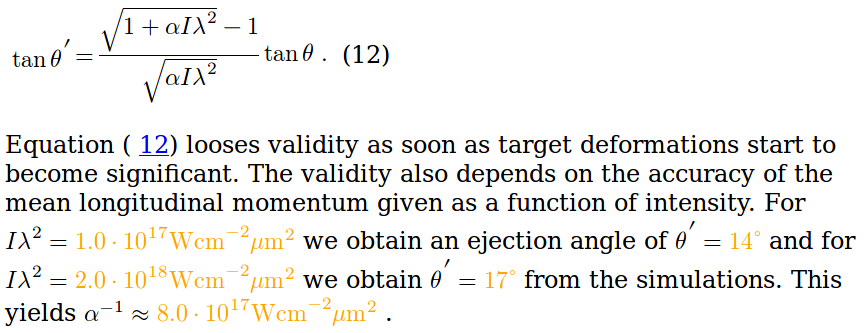
\includegraphics[width=12cm]{screenshots/highlight}}
    \caption{Highlighting Quantity Expressions in \cite{physics/9807021}}\label{fig:highlight}
\end{figure}

In the first case, the user wants to convert a unit in just one expression to an
equivalent one, say watt to horsepower. For that, she can right-click on this particular
expression and choose a target unit (e.g.  horsepower) from the list of units that are
equivalent to Watt. Figure~\ref{fig:convertone} demonstrates this and
Figure~\ref{fig:convertoneresult} displays the result of the computation.

\begin{figure}
  \begin{subfigure}{8cm}
    \fbox{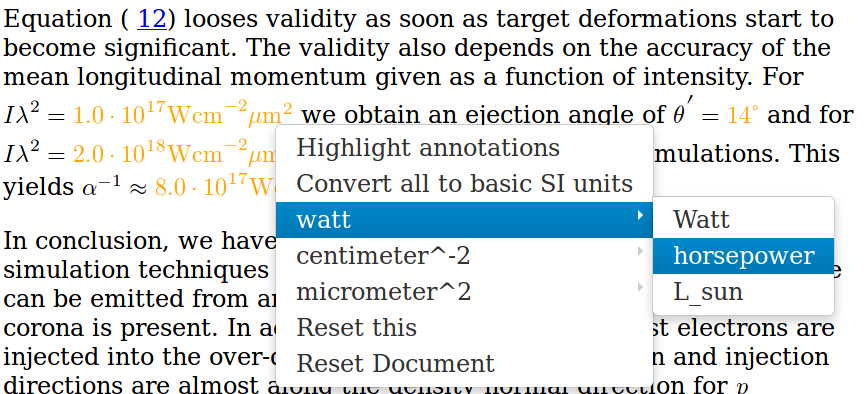
\includegraphics[width=7.5cm]{screenshots/convertone}}
    \caption{Choosing A Target Unit}\label{fig:convertone}
  \end{subfigure}
  \begin{subfigure}{7.5cm}
    \fbox{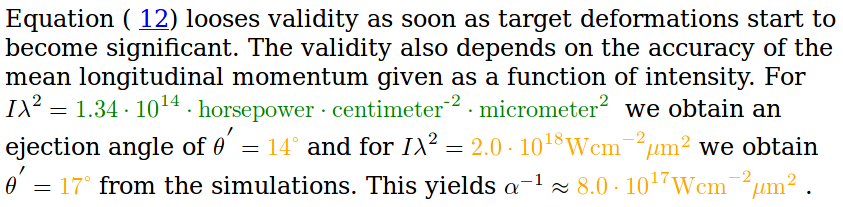
\includegraphics[width=7cm]{screenshots/convertoneresult}}
    \caption{The Result of converting one QE}\label{fig:convertoneresult}
    \fbox{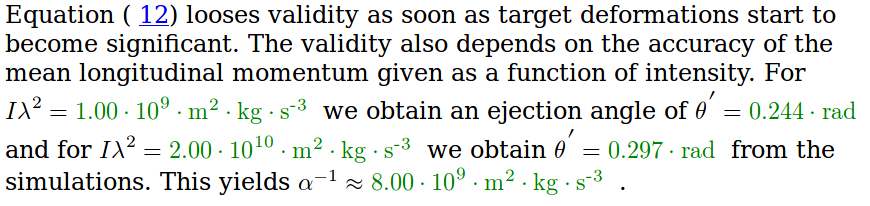
\includegraphics[width=7cm]{screenshots/si}}
    \caption{Converting a Document To SI}\label{fig:si}
  \end{subfigure}
  \caption{In-Situ Unit Conversion}\label{fig:unit-conversion}
\end{figure}

The current example only allows local conversions, but of course the user also wants
to convert units document-wide -- ideally from one system of measurement to another. 
Figure~\ref{fig:si} shows the result of a prototypical implementation, which 
converts all units to irreducible SI base units. 
This could, for instance, be extended to automatically convert all quantity
expressions in a document from imperial to metric units and vice versa. 

\subsection{A General Framework for In-Situ Computation}\label{sec:impl:general}

  A right click on a formula $F$ triggers the JOBAD menu, which has a ``compute with me''
  field, which triggers
  \begin{itemize}
  \item The \textbf{context extractor}, a function that for all the \lstinline|ci|
    elements in the content formula $C$ associated with $F$, tries to find the associated
    variable declarations by going up the parent chain of $F$ and the symbol declarations
    from the home theory -- the latter is functionality provided by the MMT system. Note
    that using the content MathML representation $C$ of $F$ gets us around disambiguation
    problems: even if the presentation of $F$ is ambiguous (e.g. by using variable or
    constant names multiple times), $C$ is not.
  \item The variable context is displayed to the user prompting instantiation in a popup
    form: the \textbf{in-situ computation manager} (see Figure~\ref{fig:compman}\ednote
    {replace this with a screenshot.}), which allows to give values for the components of
    the equation, specify actions (simplification, equation solving, \ldots) and ways of
    providing the results.\ednote{MK: we should think of more ways than ``in-place'' and
      ``footnote'' here.}\ednote{MK: the manager should eventually also give access to
      multiple computation machines.}
  \item The user-supplied values are parsed into Content MathML, inserted into $C$,
    yielding the content MathML expression $C'$, which is then shipped to the
    computational engine. Currently we only support the MMT system as a computational
    engine, but this is not a restriction, since MMT can delegate computations to engines
    like GAP, Sage, PARI, \ldots via the SCSCP protocol~\cite{ODK-D3.3}. 
  \item Finally, the result $R$ of computing $C'$ -- a content MathML expression -- is
    presented in presentation MathML and inserted into the document. \ednote{show screen
      shots of the examples from Section~\ref{sec:examples}.}
  \end{itemize}

  \begin{figure}[ht]\centering
    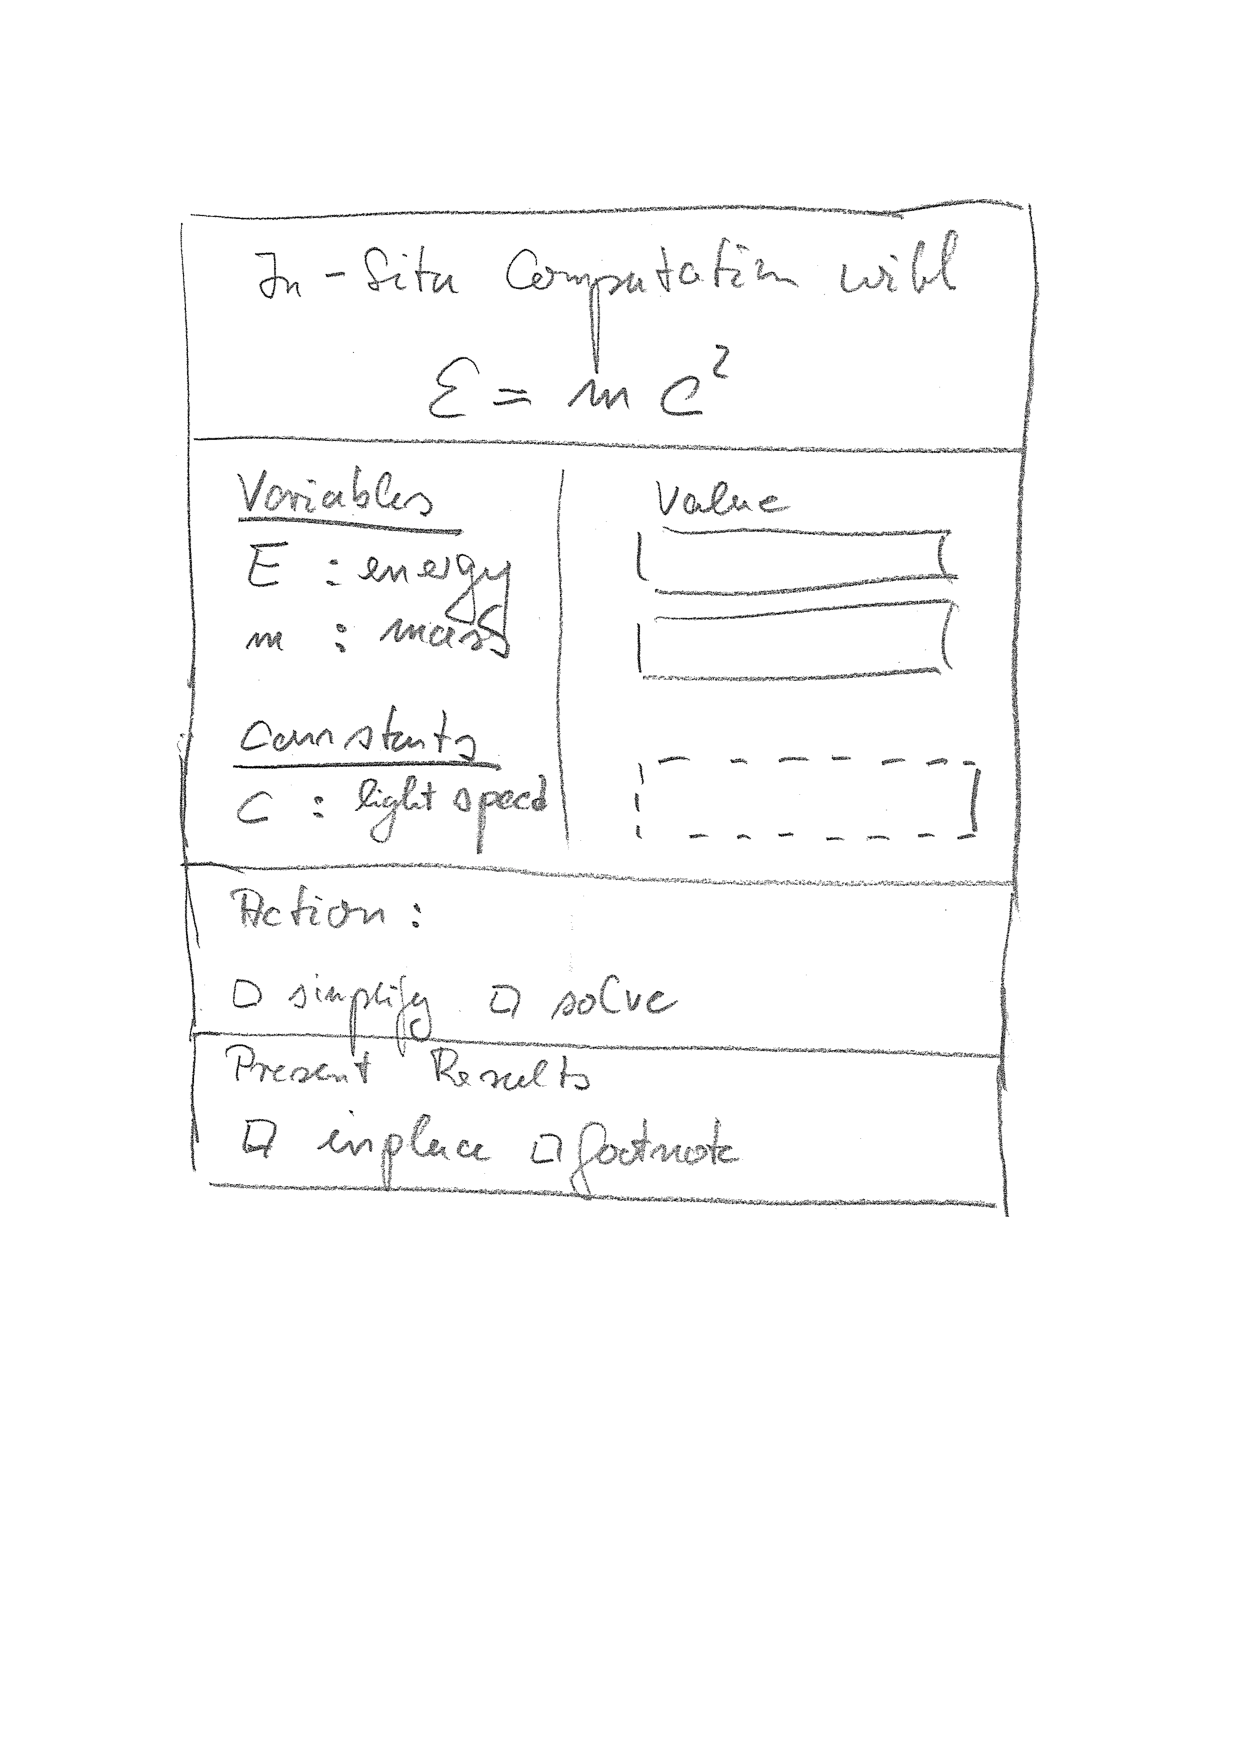
\includegraphics[width=10cm]{compman}
    \caption{In-Situ Computation Manager}\label{fig:compman}
  \end{figure}

\subsection{Code Availability, Licensing and Demos}  
\ednote{MK@TW: describe where to find things and how to see the demos. Please also get the
  information from Ulrich. I want a demo from him as well.}
  
%%% Local Variables:
%%% mode: latex
%%% TeX-master: "report"
%%% End:
